\chapter{Optimization Approaches}
\label{optapproaches}
This chapter introduces and discusses the optimization approaches that will be benchmarked later. It will start with the simple implementations and will gradually present the implementations with more performance optimizations. In \autoref{chapter:exp_eval} only the most optimized versions will be tested.
\section{Baseline float32 implementation}
\label{naivefloat}
\begin{figure}[h]
    \begin{algorithm}{setEmbeddings function from the float implementation.}{setEmbeddingsFloat}
        \begin{lstlisting}[language=C++]
bool EmbeddingSearchFloat::setEmbeddings(
        const std::vector<std::vector<float>> &input_vectors) {
    initializeDimensions(input_vectors);
    embeddings = input_vectors;
    return true;
}
    \end{lstlisting}
    \end{algorithm}
\end{figure}

\begin{figure}[h]
    \begin{algorithm}{Loop calculates the similarity for every embedding with the query.}{similarityloop}
        \begin{lstlisting}[language=C++]
for (size_t i = 0; i < embeddings.size(); ++i) {
    float sim = cosine_similarity(query, embeddings[i]);
    similarities.emplace_back(sim, i);
}
    \end{lstlisting}
    \end{algorithm}
\end{figure}

\begin{figure}[h]
    \begin{algorithm}{Naive cosine similarity function.}{naivecosinesimilarity}
        \begin{lstlisting}[language=C++]
float cosine_similarity(const std::vector<float> &a,
                        const std::vector<float> &b) {
    float dot_product = 0.0f;
    float mag_a = 0.0f;
    float mag_b = 0.0f;
    for (size_t i = 0; i < a.size(); ++i) {
        dot_product += a[i] * b[i];
        mag_a += a[i] * a[i];
        mag_b += b[i] * b[i];
    }
    return dot_product / (std::sqrt(mag_a) * std::sqrt(mag_b));
}
    \end{lstlisting}
    \end{algorithm}
\end{figure}

The naive and simple float implementation resides in the class \textit{EmbeddingSearchFloat}. In this class the embeddings vectors are set by simply copying the vectors from the load function:~\autoref{alg:setEmbeddingsFloat}. The similarities are calculated by iterating over all embeddings and comparing the similarity for each with the query. This stays the same for all searcher implementations. See~\autoref{alg:similarityloop}.
The cosine similarity for two vectors is calculated by iterating over every vector element. Then the corresponding vector elements of the input vectors are multiplied to each other. The result is then added to the dot product. After the loop we have the correct dot product value in the value \textit{dot\_product}. The cosine similarity is then derived from the dot product like its explained in \autoref{sec:cosinetodot}.
After all similarities are calculated in \autoref{alg:similarityloop}, the results are sorted by the cosine similarity and returned. Generally this version is the slowest and uses the most memory because it doesn't use any quantization to reduce memory usage or special instructions to accelerate the computation.

\section{Cosine Similarity Optimization}
Normalizing the embeddings during loading or quantization eliminates the normalization calculation during cosine calculation. This greatly decreases the FLOPs required. This saves power and can also accelerate the calculation if it's not memory bottlenecked.

\section{Quantization Methods}
\subsection{Int8 quantization}
\label{int8quant}
\begin{figure}[h]
    \begin{algorithm}{Int8 cosine similarity function.}{int8cosinesimilarity}
        \begin{lstlisting}[language=C++]
int cosine_similarity(const std::vector<int8> &a,
                      const std::vector<int8> &b) {
    int dot_product = 0;
    for (size_t i = 0; i < a.size(); ++i) {
        dot_product += a[i] * b[i];
    }
    return dot_product;
}
    \end{lstlisting}
    \end{algorithm}
\end{figure}
While the int8 quantization is not implemented without any other optimization (like AVX2 or optimized memory management) it works by multiplying each vector element by 127. The embeddings have to be normalized for this. If they are not normalized the original values can exceed -1 or 1 and cause the 8-bit integer to overflow. The loop iterating over every embedding looks like the one shown in \autoref{alg:similarityloop}. The cosine similarity is calculated by simply calculating the dot product as seen in \autoref{alg:int8cosinesimilarity}. Dividing by the magnitude of the vectors isn't necessary, because the vectors have already been normalized. Int8 embeddings use 1/4 of the memory that the float32 embeddings use. The cosine calculation is also faster, because multiplying int8 values is faster than multiplying float32 values. Another speedup factor is the vector normalization before calculating the cosine similarity. One downside is that the multiplication results of the two vector elements have to be stored in an int16 value because in the worst case you need 16bit for the result of an 8-bit int multiplication.

\subsection{Binary quantization}
\label{binaryquant}
For the binary quantization the conversion from the float value to binary is very simple. Because each vector element has to be represented by one bit, it represents negative values as \texttt{0} and positive values as \texttt{1}. Instead of just creating a vector of booleans, 64 vector elements are represented by one 64bit int value. Now the binary embeddings have 1/64 the original vector size. The algorithm that does the conversion is shown in \autoref{alg:binaryquant}. Here the vectors don't need to be normalized, because a binary vector can have just one length anyway.
Again the function iterating over every embedding and calculating the cosine similarity is like the one shown in \autoref{alg:similarityloop}.
Then we can use XNOR-based binary multiplication to build the dot product. The whole 64bit integer of the query gets XNORd with the integer from the embedding. Then popcount is used to count the ones as ones represent the matching bits. This is shown in \autoref{alg:binarycosine}. The higher the returned dot product is the more similar the vectors are.

\begin{figure}[h]
    \begin{algorithm}{Quantization of binary embeddings}{binaryquant}
        \begin{lstlisting}[language=C++]
for (size_t i = 0; i < num_vectors; ++i) { // iterate over vectors
    for (size_t j = 0; j < float_vector_size; ++j) { // vec elements
        if (float_data[i][j] >= 0) { // when float has positive val
            size_t chunk_idx = j / 64;
            size_t bit_pos = j % 64;
            embeddings[i][chunk_idx] |= (1ULL << (63 - bit_pos));
        }
    }
}
    \end{lstlisting}
    \end{algorithm}
\end{figure}

\begin{figure}[h]
    \begin{algorithm}{Cosine similarity for binary embeddings}{binarycosine}
        \begin{lstlisting}[language=C++]
int cosine_similarity(const std::vector<uint64_t> &a,
                      const std::vector<uint64_t> &b) {
    int dot_product = 0;
    for (size_t i = 0; i < a.size(); ++i) {
        // Count matching bits using XOR and NOT
        dot_product += __builtin_popcountll(~(a[i] ^ b[i]));
  }
  return dot_product;
}
    \end{lstlisting}
    \end{algorithm}
\end{figure}
\subsection{Float16 quantization}
\label{sec:float16}
The float16 quantization is implemented using the software float16 implementation from C++. All the functions are similar to the naive float32 functions. Except that the embeddings in \textit{setEmbeddings} are converted using the standard float16 constructor as seen in \autoref{alg:float16setemb}. For this implementation its only relevant to compare accuracy and memory metrics. Time based metrics will be excluded, because the float16 software implementation is very slow and most desktop/laptop processors don't support float16 natively yet.
\begin{figure}[h]
    \begin{algorithm}{Excerpt from setEmbeddings function from the float16 class}{float16setemb}
        \begin{lstlisting}[language=C++]
embeddings[i][j] = std::float16_t(input_vectors[i][j]);
    \end{lstlisting}
    \end{algorithm}
\end{figure}
% MAPPED FLOAT
\subsection{Mapped float quantization}
\label{sec:mappedfloat}
\begin{figure}[h]
    \makebox[\textwidth][c]{%
        \begin{minipage}{0.49\widefigwidth}
            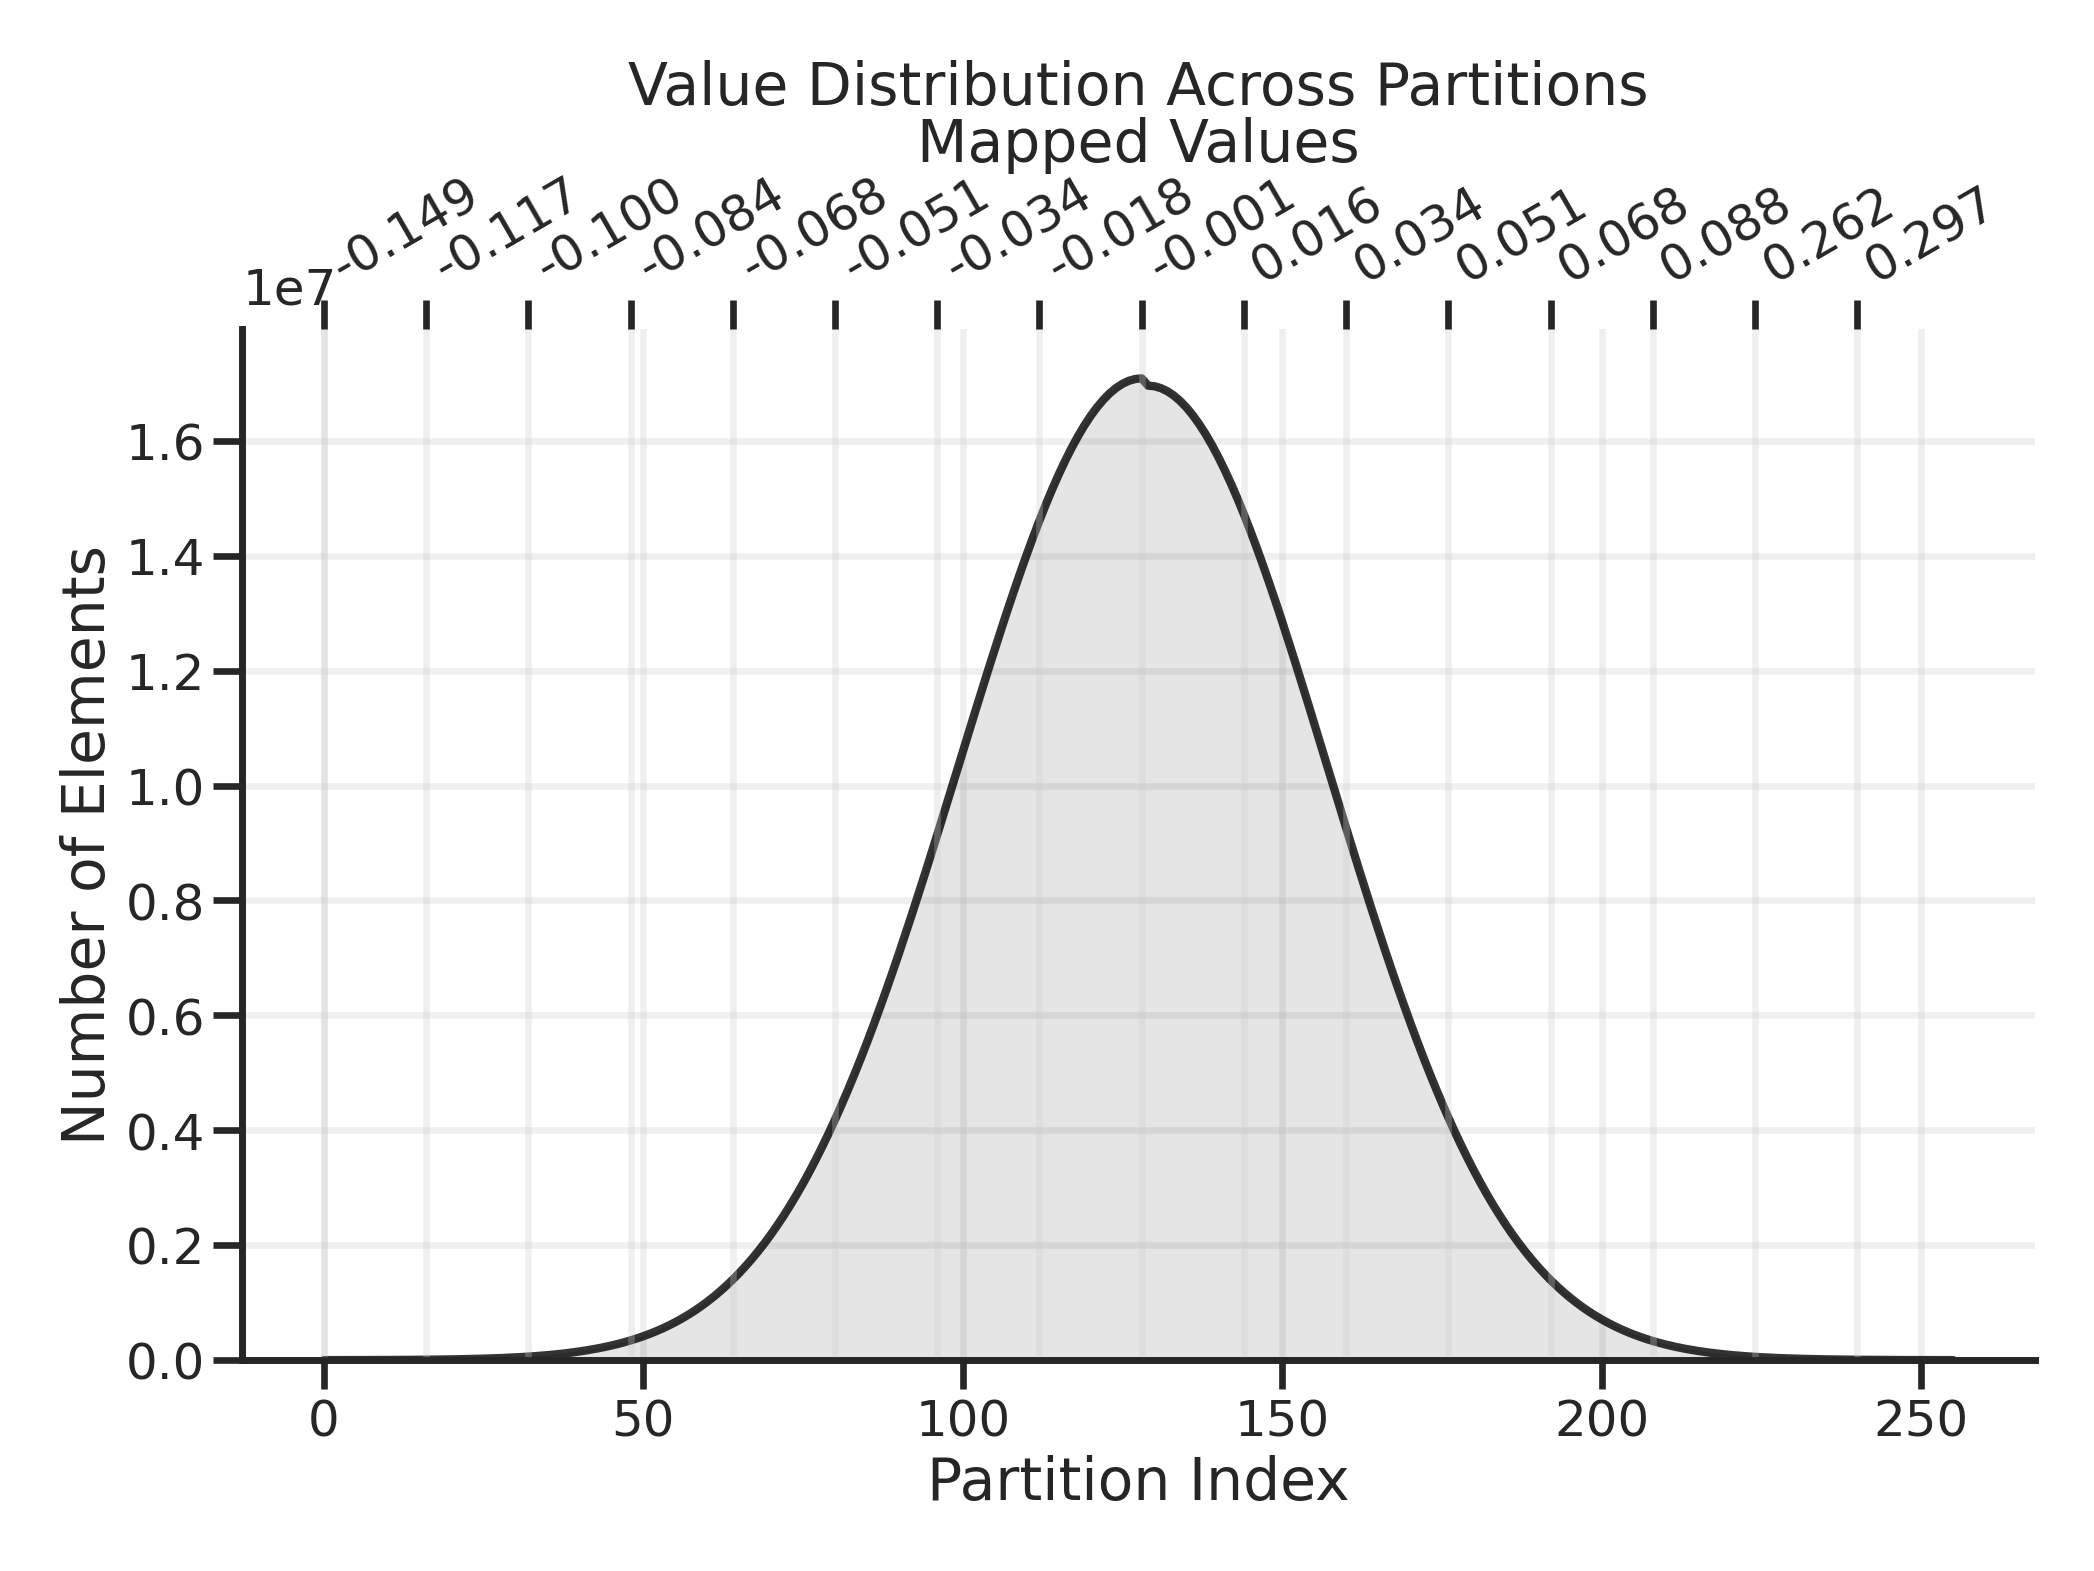
\includegraphics[width=0.49\widefigwidth]{bilder/plots/value_distribution.png}
            \vspace*{-1cm}
            \caption{\scriptsize{Value distribution of quantized test dataset}}
            \label{mfvaluedist}
        \end{minipage}
        %\hfill
        \begin{minipage}{0.49\widefigwidth}
            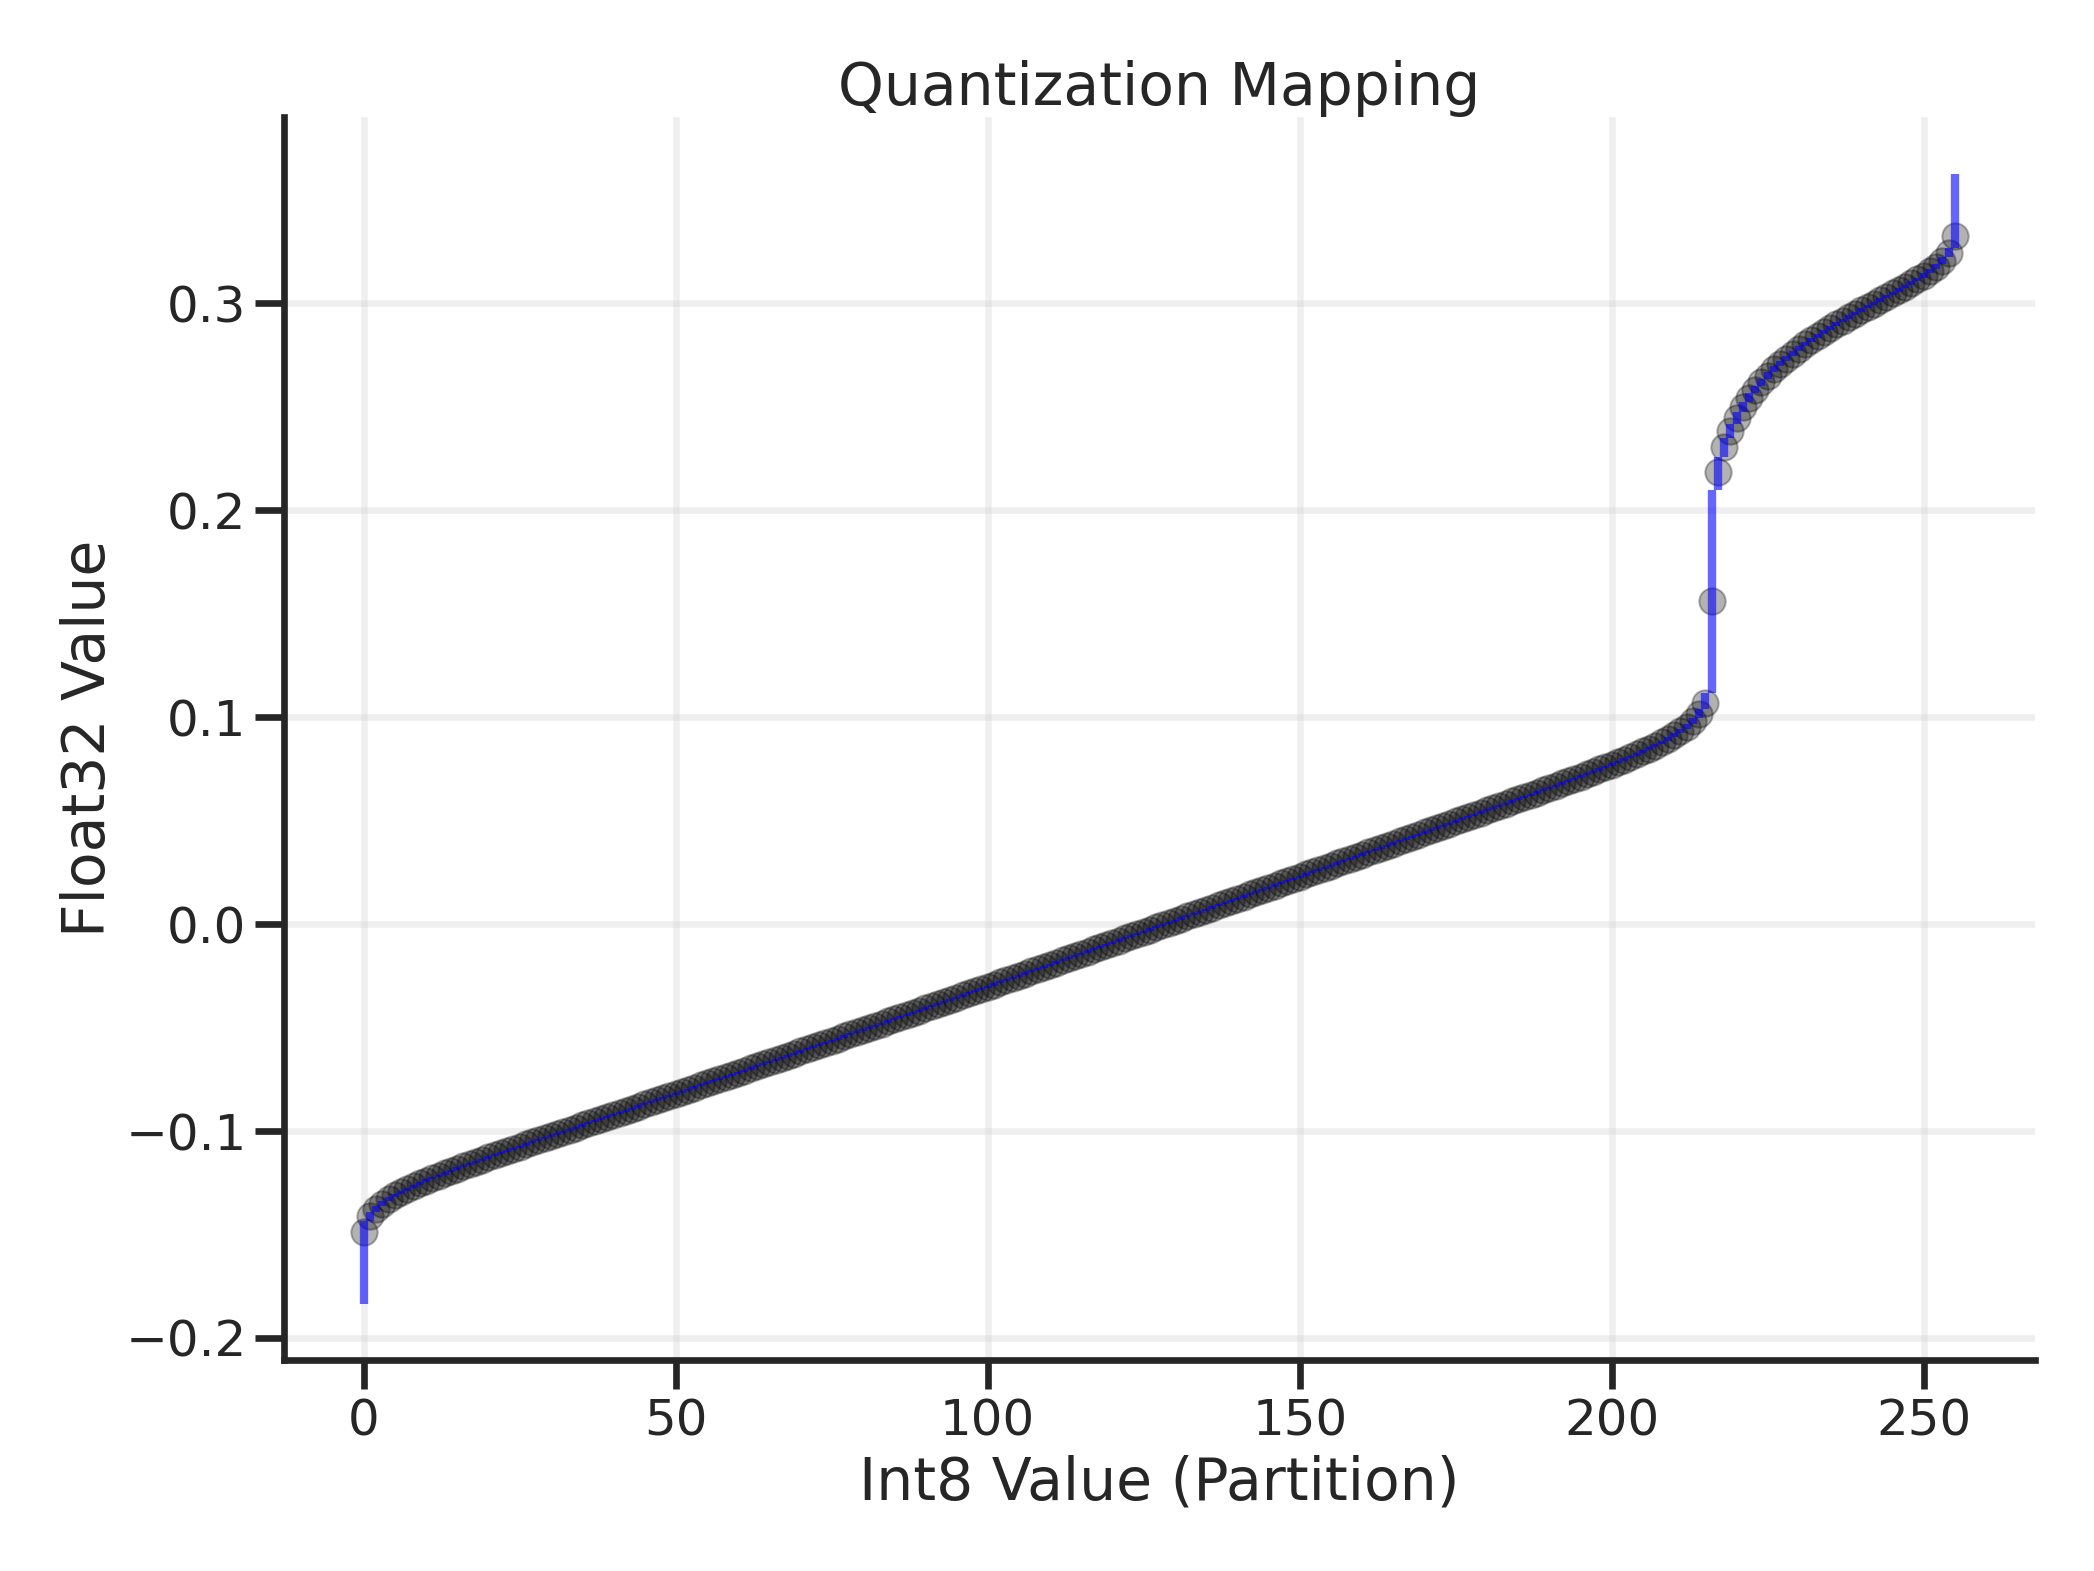
\includegraphics[width=0.49\widefigwidth]{bilder/plots/quantization_mapping.png}
            \vspace*{-1cm}
            \caption{\scriptsize{Quantization Mapping of quantized test dataset}}
            \label{mfquantmapping}
        \end{minipage}
    }
\end{figure}
The mapped float quantization uses a novel technique that combines quantization with value mapping to achieve high accuracy while reducing memory usage. Like the int8 quantization it uses 8bit integers to store the quantized values. But it doesn't just linearly map the values to the [-127, 127] range. This method analyzes the value distribution of the embedding vectors during quantization and adapts the quantized values to it.

In the first step of quantization the embedding matrix is flattened into a single array in which the float values are sorted. This gives the distribution of all values across all embeddings. For the test dataset with 1 200 000 embeddings with 1024 dimensions, this would result in 1.2 billion float values to sort.

Now the sorted values are partitioned into 256 segments using a Gaussian distribution weighting. This is implemented in the \texttt{partitionAndAverage} function:~\autoref{alg:distributionweighting}.
\begin{figure}[h]
    \begin{algorithm}{Distribution weighting}{distributionweighting}
        \begin{lstlisting}[language=C++]
double weight = std::exp(-relative_pos * relative_pos * factor);
    \end{lstlisting}
    \end{algorithm}
\end{figure}
Here \textit{relative\_pos} is the normalized position (-1 to 1). \textit{factor} controls the shape of the distribution and can be used for fine tuning. This weighting guarantees more precision in dense regions of the distribution, while also allowing outliers that are closer to -1 or 1 to keep their relatively high impact during the similarity computation.
For each partition its most important values are stored inside the \textit{PartitionInfo} struct. The average values of each partition are also stored in the \textit{mapped\_floats} array.
\begin{figure}[h]
    \begin{algorithm}{PartitionInfo and mapped\_float array}{partitioninfomappedfloatarray}
        \begin{lstlisting}[language=C++]
struct PartitionInfo {
  float start;    // First value in partition
  float end;      // Last value in partition
  float average;  // Average of all values in partition
};
alignas(32) float mapped_floats[256];
    \end{lstlisting}
    \end{algorithm}
\end{figure}
At the end of the quantization process, each float value in the original embedding is mapped to an uint8 index defined by the partitions' boundaries it fits into. The partition is efficiently searched via binary search. The cosine similarity function uses AVX2 gather instructions to efficiently load the corresponding mapped float values for the given uint8 indices as shown in~\autoref{alg:mappedfloatcosinesimilarity}.
\begin{figure}[h]
    \begin{algorithm}{Excerpt from mapped float cosine similarity}{mappedfloatcosinesimilarity}
        \begin{lstlisting}[language=C++]
__m256i indices_b = _mm256_cvtepu8_epi32(...);
__m256 values_b = _mm256_i32gather_ps(mapped_floats, indices_b, 4);
    \end{lstlisting}
    \end{algorithm}
\end{figure}
The query vector stays as is because it's kept as a float32 vector the entire time as it would make no sense to convert it to the uint8 indices and then back to float. In conclusion this method has the following advantages:
\begin{itemize}
    \item It only uses 1/4th of the memory the float32 based searchers needs.
    \item The weighted partitioning gives precise Quantization in dense areas but still can represent outliers good enough to impact the dot product.
    \item Small, 1 kB mapping table can stay in L1 cache.
    \item Gather instructions are usually to slow to make sense combining them with vector instructions. But as the mapping table stays entirely in L1 cache the latency penalty is less bad.
\end{itemize}

\section{Dimension reduction}
\label{sec:dimreduct}
Principal Component Analysis (PCA) is another approach to reduce memory usage and accelerating the search by reducing vector dimensions. The simsearch program has a function that takes the embedding matrix and a reduction factor as input. When the function is finished it will return the dimension reduced embedding matrix, the PCA-matrix and the mean vector. The latter two are required to convert search queries to the same dimension as the dimension reduced embeddings. This method uses the Eigen library to simplify the matrix and vector operations.
From now on the original vector dimension will be $d$ and $n$ is the number of embeddings. The embedding matrix will be called $M$. Logically $M$ is an $n \times d$ Matrix.

In the first step the mean vector across all embeddings is calculated and then subtracted form each vector. This centers the data around the origin and increases the PCA effectiveness.

In the next Step the $d \times d$ covariance matrix gets calculated: $Cov = \frac{(M^T \cdot M)}{n-1}$
This matrix describes the relationship between dimensions.

Now the eigenvalues and eigenvectors of the covariance matrix are calculated. The eigenvectors get sorted by descending eigenvalue magnitude. Larger eigenvalues suggest more important principal components.

Next we do the dimensionality reduction: Select top $k = d / reduction\_factor$ eigenvectors.
With these top k eigenvectors, the PCA-matrix $P$ of size $d \times k$ gets created. The original embeddings now can get dimension reduction by multiplying it with the PCA-matrix: $M_{reduced} = M \cdot P$\\
$M_{reduced}$ now has the dimensions $n \times k$.

Finally, in the last step, the vectors have to get normalized again.

\section{SIMD optimization}
\subsection{Float32 implementation with AVX2}
\label{floatimplavx2}
\begin{figure}[h]
    \begin{algorithm}{Converting float vector to AVX2}{floatvectoavx2}
        \begin{lstlisting}[language=C++]
void convertEmbeddingToAVX2(const std::vector<float> &input,
                            avx2_vector &output, size_t vector_dim) {
    for (size_t j = 0; j < vector_dim; j++) {
        size_t k = j * 8; // Each AVX2 vector holds 8 floats
        // will load 8*32bit -> input[i] .. input[i+7]
        output[j] = _mm256_loadu_ps(&input[k]);
    }
}
    \end{lstlisting}
    \end{algorithm}
\end{figure}
\begin{figure}[H]
    \begin{algorithm}{Cosine similarity for AVX2 float vectors}{cosinefloatavx2}
        \begin{lstlisting}[language=C++]
inline float _mm256_reduce_add_ps(__m256 x) {   // Sum all 8 floats in x
  __m128 high128 = _mm256_extractf128_ps(x, 1); // Get upper 4 floats
  __m128 low128 = _mm256_castps256_ps128(x);    // Get lower 4 floats
  __m128 sum = _mm_add_ps(high128, low128);     // Add hi+lo -> 4 floats
  sum = _mm_hadd_ps(sum, sum);     // Adjacent pairs -> (a+b,c+d,a+b,c+d)
  sum = _mm_hadd_ps(sum, sum);     // Final sum in lowest float
  return _mm_cvtss_f32(sum);       // Extract lowest 32-bit float
}
float cosine_similarity(const avx2_vector &a,
                        const avx2_vector &b) {
  __m256 dot_product = _mm256_setzero_ps(); // <-
  __m256 mag_a = _mm256_setzero_ps();       // <- init all 3 vars with 0
  __m256 mag_b = _mm256_setzero_ps();       // <-
  for (size_t i = 0; i < a.size(); ++i) {
    __m256 prod = _mm256_mul_ps(a[i], b[i]);        // multiply vectors
    dot_product = _mm256_add_ps(dot_product, prod); // add to running sum
    mag_a = _mm256_add_ps(mag_a, _mm256_mul_ps(a[i], a[i]));//mag_a+=a^2
    mag_b = _mm256_add_ps(mag_b, _mm256_mul_ps(b[i], b[i]));//mag_b+=b^2
  }
  float dot_product_sum = _mm256_reduce_add_ps(dot_product);
  float mag_a_sum = _mm256_reduce_add_ps(mag_a);
  float mag_b_sum = _mm256_reduce_add_ps(mag_b);
  return dot_product_sum / (sqrt(mag_a_sum) * sqrt(mag_b_sum));
}
    \end{lstlisting}
    \end{algorithm}
\end{figure}
This implementation will have the same accuracy and memory usage as the naive float implementation but it will be faster because AVX2 can multiply two vectors, consisting of 8 floats each, at once. We convert the default float vectors into AVX2 by simply loading the original vectors in 256 bit / 32 Byte steps into the AVX2 Vector as shown in \autoref{alg:floatvectoavx2}.

Computing the cosine similarity works generally like in the naive float version but with AVX2 instructions. The computation will be explained with the algorithm in \autoref{alg:cosinefloatavx2}. Line 11-13 initializes the running sums for the dot product and magnitudes. The for loop iterates over the whole vector where each element is actually an AVX2 vector with 8 float elements. Next the two vectors are multiplied. After that the product is added to the dot product. Line 17, 18 squares each vector and then adds the result to the magnitude for the corresponding vector. After the for loop the sum of all float values in the three AVX2 vectors (\textit{dot\_product}, \textit{mag\_a}, \textit{mag\_b}), also called horizontal sum, are calculated with the helper function \textit{\_mm256\_reduce\_add\_ps} in \autoref{alg:cosinefloatavx2}.

\subsection{Int8 quantization with AVX2}
\label{int8implavx2}
The conversion from float to int8 works like explained in section \autoref{int8quant}. But this time we can store 32 int8 values in one AVX2 vector. The similarity gets computet in two steps: Because the results gets stored as int16 because of the potential overflow we can actually just multiply 16 values at a time. For this we first extract the lower 128bit in line 7 and 8 and multiply in line 6. The result gets stored as 256bit value, because we extend from 16*8bit to 16*16bit during multiplication. The same happens with the higher 128 bits in line 9-11. In the last step we add the \textit{mul\_lo} and \textit{mul\_hi} products to their corresponding running sum \textit{sum\_lo} and \textit{sum\_hi}. After the loop we build the horizontal sum of the two running sum vectors.

\begin{figure}[h]
    \begin{algorithm}{Cosine similarity for int8 with AVX}{cosineint8avx2}
        \begin{lstlisting}[language=C++]
uint cosine_similarity(const avx2i_vector &a,
                       const avx2i_vector &b) {
  __m256i sum_lo = _mm256_setzero_si256();// Accum. for lower 128 bits
  __m256i sum_hi = _mm256_setzero_si256();// Accum. for upper 128 bits
  for (size_t i = 0; i < a.size(); ++i) { // 32 elements per iteration
    __m256i mul_lo = _mm256_mullo_epi16(  // extr and mult lower 128 bits
        _mm256_cvtepi8_epi16(_mm256_extracti128_si256(a[i], 0)),
        _mm256_cvtepi8_epi16(_mm256_extracti128_si256(b[i], 0)));
    __m256i mul_hi = _mm256_mullo_epi16(  // extr and mult upper 128 bits
        _mm256_cvtepi8_epi16(_mm256_extracti128_si256(a[i], 1)),
        _mm256_cvtepi8_epi16(_mm256_extracti128_si256(b[i], 1)));
    sum_lo = _mm256_add_epi32(sum_lo, // Accum. into 32bit to prev overfl
               _mm256_madd_epi16(mul_lo, _mm256_set1_epi16(1)));
    sum_hi = _mm256_add_epi32(sum_hi, // Accum. into 32bit to prev overfl
               _mm256_madd_epi16(mul_hi, _mm256_set1_epi16(1)));
  } // horizontal sum gets built and returned here
}
    \end{lstlisting}
    \end{algorithm}
\end{figure}

\subsection{Binary quantization with AVX2}
\label{binaryquantavx2}
\begin{figure}[h]
    \begin{algorithm}{Cosine similarity for binary with AVX}{cosinebinaryavx2}
        \begin{lstlisting}[language=C++]
int EmbeddingSearchBinaryAVX2::cosine_similarity(const avx2i_vector &a,
                                                 const avx2i_vector &b) {
  int dot_product = 0;
  __m256i all_ones = _mm256_set1_epi32(-1); // set every bit to 1
  for (size_t i = 0; i < a.size(); ++i) {
    __m256i result = _mm256_xor_si256(a[i], b[i]); // XOR
    result = _mm256_xor_si256(result, all_ones);   // NOT
    uint64_t *result_ptr = reinterpret_cast<uint64_t *>(&result);
    dot_product += __builtin_popcountll(result_ptr[0]); // sum all 64 bit
    dot_product += __builtin_popcountll(result_ptr[1]); // popcounts for
    dot_product += __builtin_popcountll(result_ptr[2]); // 256 bit result
    dot_product += __builtin_popcountll(result_ptr[3]);
  }
  return dot_product;
}
    \end{lstlisting}
    \end{algorithm}
\end{figure}
Just like in \autoref{binaryquant} we just store the sign of the float embeddings. This time we can store 256 binary values in one AVX2 vector. Cosine similarity is computed by using XOR on both 256 bit vectors and then using XOR with a vector full of ones on the result. This flips every bit of the result. After that we have the XNOR result. We have to use \textit{popcountll} four times because each can only build the popcount of 64 bits. See \autoref{alg:cosinebinaryavx2}.

\subsection{Optimized float32 implementation with AVX2}
\label{floatoavx2}
Like explained in \autoref{memorymanagement} the optimized implementation uses manually managed memory to store the embeddings. The embeddings are set using memcpy.
% The cosine similarity works different (see \autoref{alg:cosinefloatoavx2}): Here the similarity function only gets a pointer to the vectors.
% Furthermore, the function expects both vectors to be normalized already. This way it doesn't have to calculate that magnitudes of the vectors, which also saves some computation time.
% In addition to this loop unrolling is used. One loop iteration works through 8 vectors instead of one. Although modern CPUs and compilers can unroll loops on their own it is implemented it manually here. The unroll factor is 8. That means 16 AVX vectors are loaded per iteration, which makes perfect use of the 16 256-bit AVX registers \cite{intel64manual}.
% Beyond that line 20-23 use a prefetching instruction to preload vectors into cache that will be accessed within a few loop iterations. This can also help, especially if it's fine-tuned for the used hardware \cite{prefetching}.
% Finally, this implementation also uses fused multiply-add, which has the benefit of being faster, more accurate due to less rounding and being more predictable \cite{fma}.
% At last the horizontal sum is calculated the same way the unoptimized AVX2 version does \autoref{floatimplavx2}.
A key optimization of this implementation is the use of strided memory access which increases memory bandwidth in combination with a more efficient vector loading strategy. This seems to be contrary to common knowledge, because sequential memory access should always be preferred it was also tested in isolation here \autoref{section:stridedmembwtest}.
The stride distance automatically gets adapted to the vector size as the stride length being a multiple of 4 KB seems to give the highest memory bandwidth. A reason for this could be the systems' page size, which is 4 KB. So accessing multiple pages at once could increase the bandwidth. Another reason could be memory interleaving.
This implementation also uses fused multiply-add (FMA), which has the benefit of being faster and more accurate due to less rounding and being more predictable.~\cite{fma}

The optimized vector loading leverages the fact, that the query vector stays the same across all comparisons. The result of this is just 7 loads (1 for query, 6 for embeddings) for 6 FMA instructions instead of 12 loads (6 for query, 6 for embeddings) for the same amount of FMA instructions. The loaded part of the query vector can also stay in one register while being multiplied with the 6 embeddings. This can be seen in \autoref{alg:cosinefloatoavx2}
Additionally, the regular pattern of 7 loads followed by 6 FMA instructions allows the CPU to better predict and optimize instruction execution.
The function expects both vectors to be normalized already. This way it doesn't have to calculate that magnitudes of the vectors, which also saves some computation time.

\begin{figure}[h]
    \begin{algorithm}{Cosine similarity for optimized AVX2 float vectors}{cosinefloatoavx2}
        \begin{lstlisting}[language=C++]
inline void cosine_similarity_optimized(
    const float *vec_a, float *sim, float *emb_ptr[]) {
  __m256 sum[NUM_STRIDES] = {_mm256_setzero_ps()}; // sum for all embeds
  __m256 a;              // 1 query
  __m256 b[NUM_STRIDES]; // load NUM_STRIDES(=6) embeddings at once
  for (int i = 0; i < padded_dim; i += 8) {
    a = _mm256_load_ps(vec_a + i);        // load query vec
    b[0] = _mm256_load_ps(emb_ptr[0] + i);//emb_ptr[0] pnts to curr. vec
    // do the same for indices 2,3,4 ...
    b[5] = _mm256_load_ps(emb_ptr[5] + i);//pnts to 5*strd_dst vec ahead
    sum[0] = _mm256_fmadd_ps(a, b[0], sum[0]); // FMA: sum += a * b[0]
    // do the same for indices 2,3,4 ...
    sum[5] = _mm256_fmadd_ps(a, b[5], sum[5]); // FMA: sum += a * b[5]
  } // compute horizontal sum for each sum and write to sim array ...
}
    \end{lstlisting}
    \end{algorithm}
\end{figure}
In \autoref{alg:embsearchloatoavx2} can be seen how the \textit{embedding\_search} function prepares the array of pointers to the vectors \textit{STRIDE\_DIST} apart (for loop line 6-8).
The loop starting at line 1 increments the index by \textit{NUM\_STRIDES * STRIDE\_DIST}, because that's the distance the inner loop (line 3-11) covers.
\begin{figure}[h]
    \begin{algorithm}{Excerpt from embedding\_search function of optimized AVX2 float class}{embsearchloatoavx2}
        \begin{lstlisting}[language=C++]
for (size_t i = 0; (i + (NUM_STRIDES * STRIDE_DIST) - 1) < num_vectors;
       i += (NUM_STRIDES * STRIDE_DIST)) { // inc by total dist covered
    for (size_t j = i; j < (i + STRIDE_DIST); j++) { // by inner loop
      float sim[NUM_STRIDES] = {}; // cosine fn writes result into this
      float *emb_ptr[NUM_STRIDES]; // arr of ptrs to vectors STRIDE_DIST
      for (int k = 0; k < NUM_STRIDES; k++) { // apart
        emb_ptr[k] = get_embedding_ptr(j + k * STRIDE_DIST);
      }
      cosine_similarity_optimized(query_aligned.data(), sim, emb_ptr);
      // store results...
    }
  }
    \end{lstlisting}
    \end{algorithm}
\end{figure}

\subsection{Optimized int8 implementation with AVX2}
\label{sec:optint8avx2}
The cosine function of this is mostly similar to the one already presented in \autoref{int8implavx2}. It uses the memory in the same way as the optimized float32 implementation in \autoref{floatoavx2}.
\subsection{Optimized binary implementation with AVX2}
\label{sec:optbinaryavx2}
\begin{figure}[h]
    \begin{algorithm}{Cosine similarity for optimized AVX2 binary vectors}{cosinebinaryoavx2}
        \begin{lstlisting}[language=C++]
int32_t cosine_similarity_optimized(const __m256i *vec_a,
                                    const __m256i *vec_b) const {
  // prefetch 2 cache lines for 4 vectors 10 loops ahead
  _mm_prefetch(vec_a + 4 * 10, _MM_HINT_T0);
  _mm_prefetch(vec_a + 4 * 10 + 2, _MM_HINT_T0);
  __m256i all_ones = _mm256_set1_epi32(-1);
  __m256i xor_result[4];
  xor_result[0] = _mm256_xor_si256(vec_a[0], vec_b[0]);      // XOR
  xor_result[0] = _mm256_xor_si256(xor_result[0], all_ones); // NOT
  xor_result[1] = _mm256_xor_si256(vec_a[1], vec_b[1]);      // XOR
  xor_result[1] = _mm256_xor_si256(xor_result[1], all_ones); // NOT
  // do the same for indices 2 and 3
  // popcnt lookup is faster than harley seal and builtin
  return counter.popcnt_AVX2_lookup( // optimized version using AVX2
      reinterpret_cast<const uint8_t *>(xor_result),
      4 * sizeof(__m256i));
}
    \end{lstlisting}
    \end{algorithm}
\end{figure}
\noindent The embeddings are set similarly to method described in \autoref{binaryquant} and \autoref{binaryquantavx2}. Like the optimized float implementation in \autoref{floatoavx2}. This cosine implementation also uses loop unrolling and manual prefetching. The XNOR based binary multiplication matches the previous one in \autoref{binaryquantavx2}. But a big improvement is the usage of 256-bit popcount algorithm implemented with AVX2 instructions, which was developed by \citeauthor{Mu_a_2017}.~\cite{Mu_a_2017} Cosine similarity algorithm can be seen here \autoref{alg:cosinebinaryoavx2}.

\section{Two-step search with rescoring}
\label{sec:twostep}
The two-step approach uses a fast but lower accuracy search first to filter for candidates. Then a full accuracy search is done on these candidates. The top results from the second search are the final result. The goal of this method is to combine the speed of the lower accuracy search with the high accuracy of full precision search. The amount of documents the first search retrieves can be tuned with the rescoring factor. The amount of documents retrieved by the first searcher is defined by $rescoring\_factor * k$. In the second step the top $k$ documents will be retrieved. There are two two-step searchers that will be tested: The first is implemented using the optimized versions of the binary and float32 searchers displayed in \autoref{alg:twostep}. The second one uses the optimized binary searcher and the mapped float searcher for rescoring.

\begin{figure}[h]
    \begin{algorithm}{Two-step search with binary searcher and full precision searcher}{twostep}
        \begin{lstlisting}[language=C++]
// Binary search for initial filtering
auto binary_results = binary_avx2_searcher->similarity_search(
    queryBinaryAvx2,     // Binary query vector
    k * rescoring_factor // Get more candidates for rescoring
);
// Full precision rescoring
auto avx2_results = avx2_searcher->similarity_search(
    query,              // Original float query
    k,                  // Final number of results
    binary_results      // Pre-filtered candidates
);
        \end{lstlisting}
    \end{algorithm}
\end{figure}